%!TEX root = main.tex
%%%%%%%%%%%%%%%%%%%%%%%%%%%%%%%%%%%%%%%%%%%%%%%%%%%%%%%%%%%%%%%%%%
\chapter{Threat model, guarantees, assumptions}
\label{sec:threat}
%%%%%%%%%%%%%%%%%%%%%%%%%%%%%%%%%%%%%%%%%%%%%%%%%%%%%%%%%%%%%%%%%%

\begin{figure}[t]
  \centering
  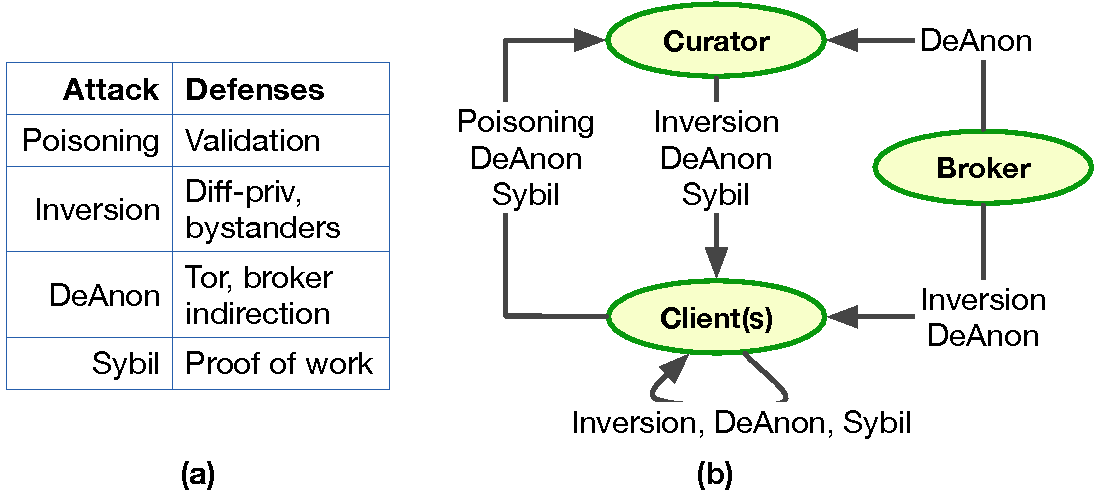
\includegraphics[width=.9\linewidth]{fig/who-attacks-who}
  \caption{(a) Attacks/defenses in TorMentor. (b) Threat model: an
    edge is an attack by source against target(s).}
  \label{fig:threatmodel}
\end{figure}

%\subsection{Threat Model}

We realized brokered learning in a system called \emph{TorMentor},
which uses differentially private distributed SGD~\cite{Song:2013} to
train a model in an anonymous multi-party setting. We select 
Tor~\cite{Dingledine:2004} as the anonymous communication network for
TorMentor. TorMentor is designed to counter malicious curators and
malicious clients who may attempt to gain additional information 
(information leakage) about others or negatively influence the
learning process (poisoning). The honest-but-curious broker coordinates
the learning process, but is \emph{not} trusted with the identity nor
the data of users.

Clients and curators do not attack the broker itself, rather they aim
to attack other curators, other clients, or the outcome of the learning
process. Brokers are also untrusted in the system: the client and
curator APIs protect them from potential broker attacks. 
Figure~\ref{fig:threatmodel} overviews TorMentor's threat model with
attacks/defenses and who can attack who and how.

%% : clients can be attacked by curators or other clients
%% through inversion attacks, curators can be attacked by clients through
%% poisoning attacks, and curators and clients can use sybils to attack
%% other users.

\textbf{Deanonymization.} For anonymous communication to and from the
broker we assume a threat model similar to Tor~\cite{Dingledine:2004}:
an adversary has the ability to observe and control some, but
not all of the network. Adversaries may attempt to observe Tor traffic
as a client or as a broker in the network~\cite{Murdoch:2005,
Evans:2009, Johnson:2013}. Adversaries can also influence traffic
within Tor through their own onion router nodes, which do not
necessarily need to be active TorMentor clients. 

\textbf{Poisoning attacks.} In our threat model, poisoning attacks are
performed by clients against shared models. After a curator defines a
model, adversarial clients can use the defined learning objective to
craft adversarial samples that oppose the objective. We assume that
adversaries generate these adversarial samples using a common strategy
such as label flipping~\cite{Biggio:2012}, and join the training
process and poison the model by influencing its prediction
probabilities.

\textbf{Inversion attacks.} We assume that adversaries can target a
specific client victim who they know is using the system. Inversion
attacks can be executed from a variety of points: the adversary may be
administering the broker, the adversary may curate a model that the
victim joins, or the adversary joins model training as a client,
knowing that the victim has also joined. Although the broker does not
expose model confidence scores in the model prediction API, which are a
key piece of information for performing inversion attacks in a
black-box setting~\cite{Fredrikson:2015}, our threat model grants
adversaries white-box access to the model internals, which is more
powerful than a traditional model inversion attack. 

In TorMentor, adversarial clients have access to the global model and
can infer confidence scores or gradient step values by carefully
observing changes to the global model and reconstructing a copy of the
victim's local model. This attack is similar to a model stealing
attack~\cite{Tramer:2016}: after stealing an accurate approximation of
a victim's local model, an adversary can mount an inversion attack on
the approximation to reconstruct the victim's training examples.

\textbf{Sybil attacks.}  Since clients and curators join the system
anonymously, they can generate sybils, or multiple colluding virtual
clients, to attacks the system~\cite{Douceur:2002}. In federated
learning, all users are given an equal stake in the system, and
thus sybils make poisoning and inversion attacks linearly easier to
perform.

\section{Security guarantees} 

TorMentor guarantees that curator and client identities remain
anonymous to all parties in the system by using an anonymous
communication network. Our prototype uses Tor and provides the same
guarantees as Tor, however, it can use other anonymous
messaging systems~\cite{Vuvuzela:2015, Riposte:2015}. For example, since
Tor is susceptible to timing attacks, an adversary could target a
client by observing its network traffic to de-anonymize its
participation in the system. 

TorMentor exposes a small, restrictive API to limit a user's influence
on the system. TorMentor alleviates the risk of poisoning attacks and
inversion attacks by allowing clients to specify $k$, the minimum
number of clients required for training. When a client joins the
system, they are able to specify the number of other clients required
in the system, which TorMentor guarantees will be honored. Clients
also locally use differential privacy to further protect their privacy.
Both parameters are defined by the client, guaranteeing that clients (and not
the curator) controls this accuracy-privacy tradeoff.

%% The training process in
%% brokered learning is the stage in which the most information is
%% revealed, and in restricting the settings by which the process occurs,
%% isolating and attacking a victim becomes more difficult.

TorMentor prevents sybils through proof of work, similar to the Bitcoin
protocol~\cite{Nakamoto:2009}. This mechanism makes it expensive,
though not impossible, to mount a sybil attack. Proof of work is
implemented at two points: proof of work as a prerequisite for system
admission, and proof of work as a prerequisite for contributing to the
model.

%%%%%%%%%%%%%%%%%%%%%%%%%%%%
\section{Assumptions}
%%%%%%%%%%%%%%%%%%%%%%%%%%%%

We assume that the only means to access information within the system
is through the APIs defined in Section~\ref{sec:design}. A TorMentor
instance and its corresponding brokers are exposed as a hidden service
with a public \textit{.onion} domain. We assume that this 
\textit{.onion} becomes a widely known and trusted domain\footnote{To
build further trust the TorMentor service can use an authoritatively
signed certificate.}.

We use proof of work to defend against sybils and therefore assume that
the adversary does not have access to more than half of the
computational power relative to the total computational power across
all users in an instance of the TorMentor training 
process~\cite{Back:2002}.

We make the same assumptions as Tor~\cite{Dingledine:2004}; for
example, we assume that an adversary does not control a large fraction
of nodes within the Tor network. %; this is required to secure
%anonymity. % for users in our system.
